\chapter{Introduction}
\label{chp:introduction} 

This section is intended to provide an overview of the contents and context of this report. The first part of this section gives a brief introduction to the field of mobile autonomous robotics and computer vision, as well as the benifits and potential applications for this technology. The robot system and tools used in the project is presented in subsection \ref{}. Lastly, each of the following sections will given short introductions.




\section{Mobile Autonomous Robotics and Computer Vision}

Put the task into a larger context. Bring in some points on the societal impact of autonomous robotics and the increased potential of mobile robotics.  

The field of computer vision has seen an enormous growth over the last few decades - not only in scale, but in accessibility and capability as well. As a consequence of this recent growth, tapping into the field of computer vision is bound to reveal applications that are useful for a mobile autonomous maintenance robot. Recent discoveries within computer vision includes robust feature recognition and object detection, face detection and video processing. The latest great additions to the field are Big Data and Artificial Intelligence.

\section{System Overview}

The mobile robot being worked on in this project is shown in figure \ref{fig:RobotFront}. The manipulator arm  has been used in previous projects on robotic maintenance, and it was placed on the mobile platform during the master thesis of Petter Aspunvik. This section provides a short description of the systems used in this project and other surrounding equipment. If a more detailed description of the robot and it's equipment is required, consult the thesis of Aspunvik \cite{aspunvik}.

\subsection{The Robot} 

The robot in its current state is the result of several preceeding projects, where the master thesis of Petter Aspunvik \cite{aspunvik} and Mikael Berg \cite{berg} are the most recent contributions. 

\begin{figure}
\centering
 \begin{subfigure}[b]{0.3\textwidth}
        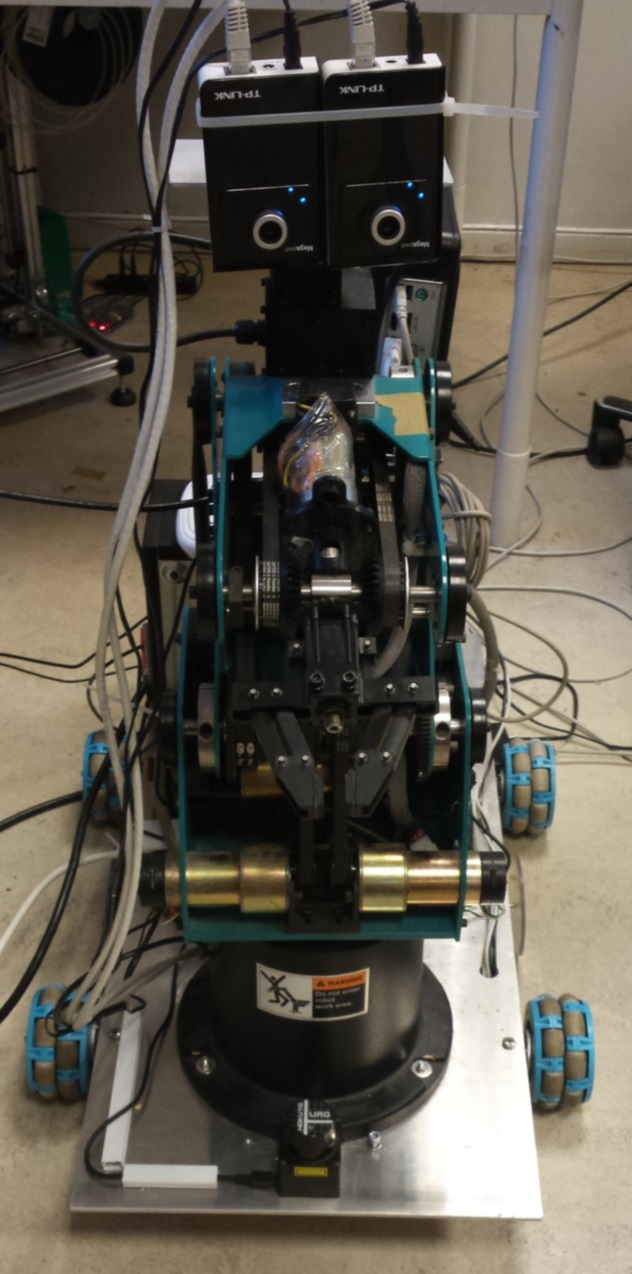
\includegraphics[width=\textwidth]{Robot_front}
        \caption{Front view.}
        \label{fig:RobotFront}
    \end{subfigure}
    \begin{subfigure}[b]{0.65\textwidth}
        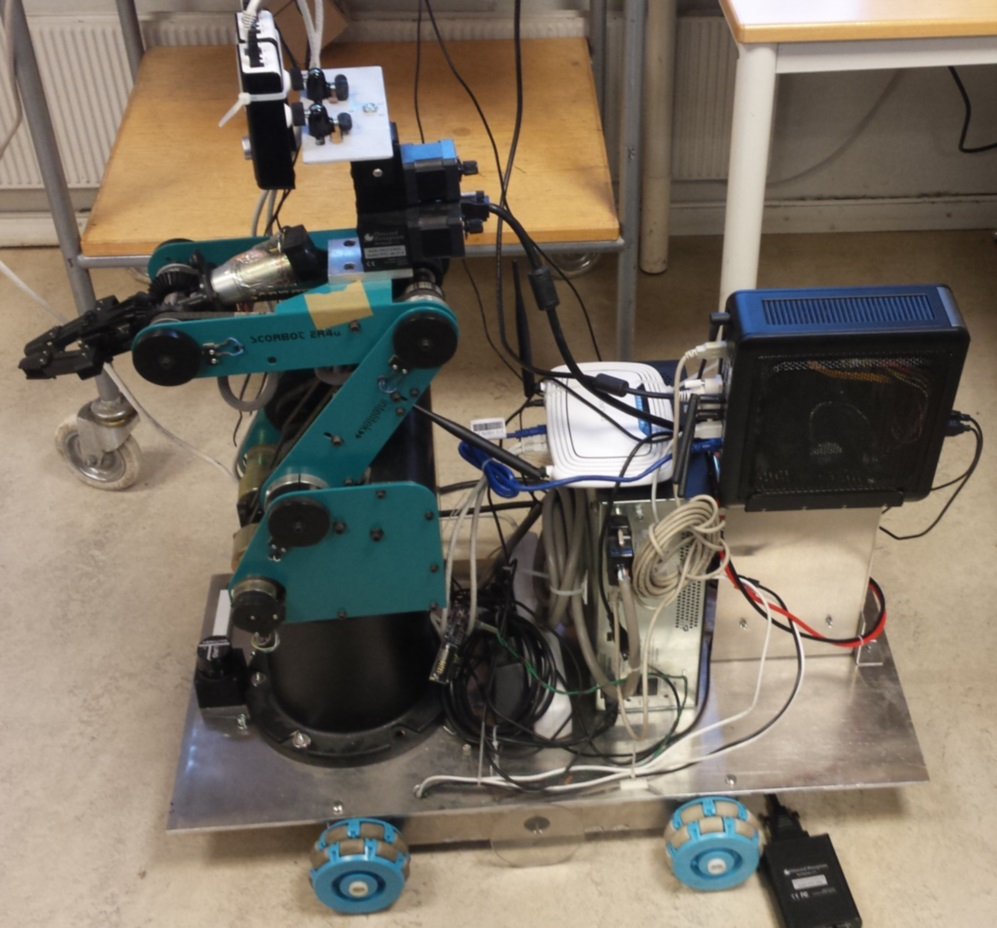
\includegraphics[width=\textwidth]{Robot_side}
        \caption{Side view.}
        \label{fig:RobotSide}
    \end{subfigure}
    \caption{\label{fig:RobotView}The robot used in the project.}
\end{figure}

\paragraph{Propulsion}

The steel chassis of the robot stands upon four omni-wheels. The wheel pairs are placed in parallel, making the vehicle uncontrollable along the lateral axis. Each wheel is powered by an electrical motor and motor driver. The motor drivers are controlled with pulse width modulation by an evaluation board from Atmel (Xmega A3BU).  

\paragraph{Sensors}

The robot has been outfitted with several sensors over the course of previous projects. These are:
\begin{itemize}
	\item Two odometer wheels with encoders. One on each side. 
	\item Two infrared distance sensors. 
	\item A LIDAR (Light Detection and Ranging).
	\item Two IP-cameras.
\end{itemize} 

Only the cameras were used in this projects. 

\paragraph{Robot Arm}

A robot arm, SCORBOT-ER 4u from Intelitek, is monted on the wagon. It is intended for educational use in the context of automation and work cells. The robot has five rotation joints plus a servo gripper at the outer joint. Control of the robot in this project is done from the on-board computer on the wagon, which is connected to the robot arm through a USB cable. 


\subsection{Project Set-up}

Vanishing points and stereo vision are the main topics in this report. The stereo vision portion consist of the two IP cameras, a pair of wireless routers and a remote computer. The remote computer can be any computer which is able to run \gls{opencv} and receive video feed from the camera pair. The vanishing point detector is simply a desktop application which accesses a web camera. Both the stereo vision and vanishing point detector applications have been developed with Qt and run on Windows 7.

\begin{figure}
	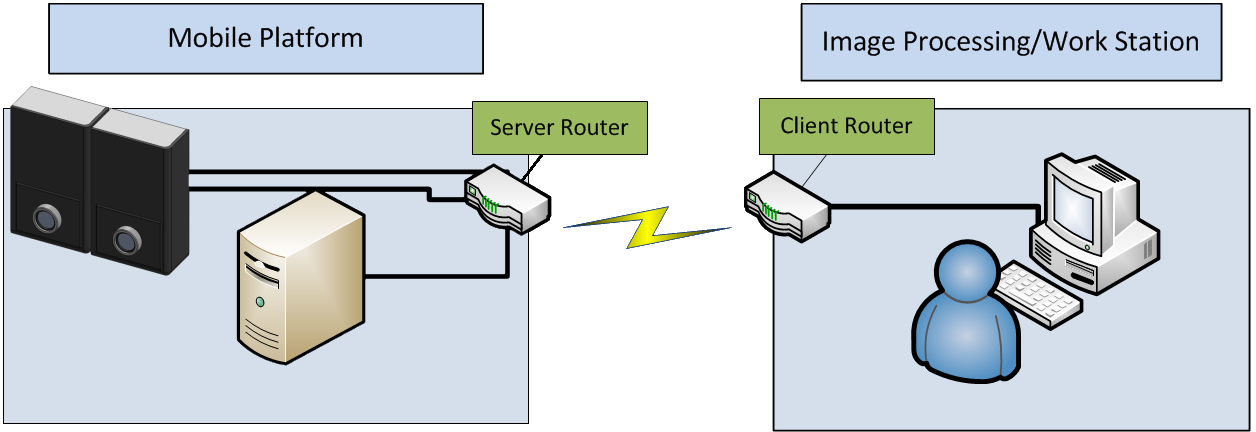
\includegraphics[width=1\textwidth]{hardwareSetup_cropped}
	\caption{\label{fig:hardware}Stereo vision set-up.}
\end{figure}

\section{Report Structure}
How the report is structured, and a very brief description of the contents in each section.